\chapter{Background}
\label{ch:bg}
This chapter details the theoretical background of clean animation frame vectorization.  \Cref{sec:bg.vec} gives an overview of both raster and vector images as well as the process of vectorization, i.e., converting raster images to vector images. \Cref{sec:anime.prod} describes the process for hand-drawn limited animation in more detail. \Cref{sec:bg.dl} explains deep learning, which is the technique used in this work to develop an automatic clean animation frame vectorization method.

\section{Vectorization}
\label{sec:bg.vec}

In a digital context, images can be  represented using either \emph{raster} or \emph{vector} data formats. These are introduced in \Cref{sec:bg.vec.raster,subsec:bg.vector}, respectively. This work is concerned with \emph{image vectorization}, i.e., the conversion of raster images into corresponding vector images, which is described in \Cref{sec:vec}.

\subsection{Raster Images}
\label{sec:bg.vec.raster}

\begin{figure}
    \centering
    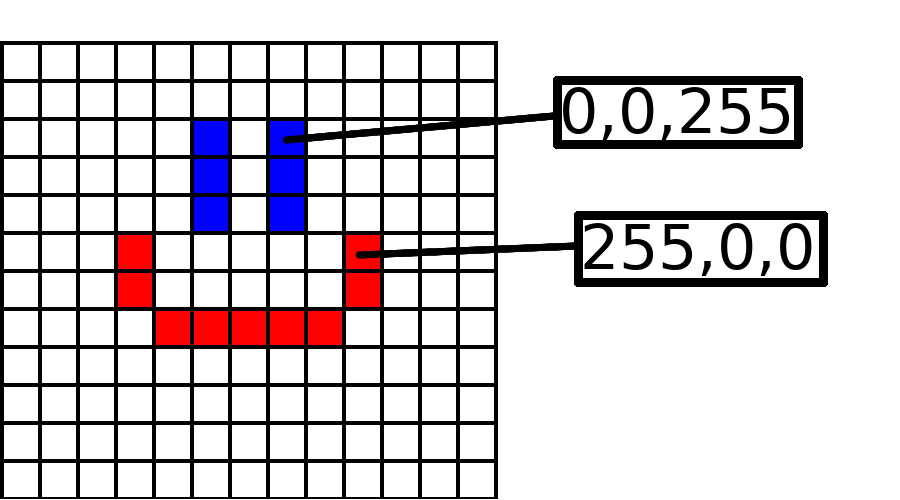
\includegraphics{graphics/raster_color_ex.png}
    \caption{Example of an image represented using a raster of 13x12 pixels. Notice that color information is stored explicitly per pixel.}
    \label{fig:raster-color-ex}
\end{figure}

Digital visual data are most commonly represented using \emph{raster} data formats. Raster images store visual data as a \emph{raster}, a 2-dimensional grid of uniformly sized squares. Each of these squares can be referred to as \emph{pixel} and is defined by its location and its color.

\begin{figure}
    \centering
    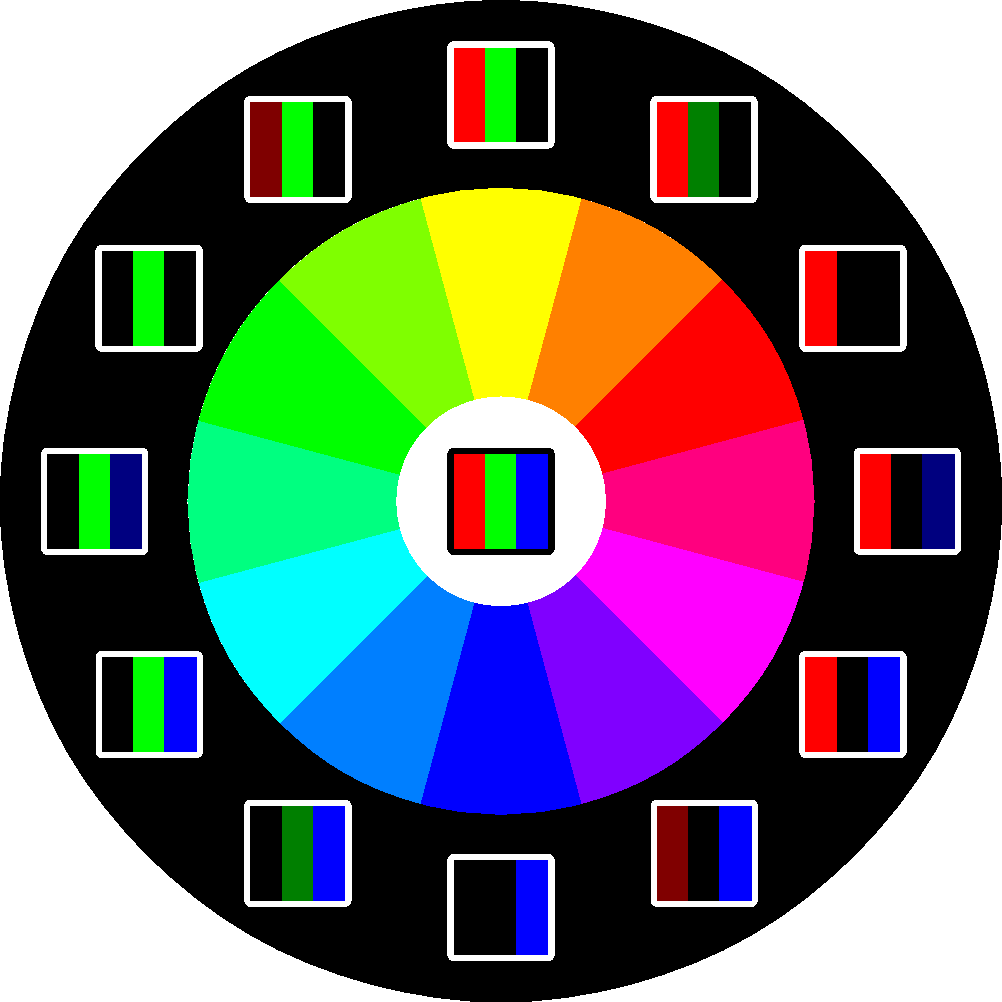
\includegraphics[width=0.5\textwidth]{graphics/RGB_color_wheel_pixel_30.pdf}
    \caption{A color wheel exemplifying the \gls{rgb} color model. The box next to each color displays the intensities of the red, green and blue component respectively (with black indicating zero intensity). The three components are added in order to produce the displayed color. Created by \citet{nemethcolorwheel}.}
    \label{fig:rgb}
\end{figure}

Raster images can be naively stored using numerical two-dimensional arrays or matrices. The pixels location in the array is directly mapped to the location on the grid (and therefore on the display). This way, the only information that needs to be stored explicitly for each pixel is its color. Usually, a color is defined using a \emph{color model} such as the \gls{rgb} or the CMYK model. In the case of \gls{rgb}, a color is defined as the intensity of each of the components red, green and blue. These components are then mixed according to their respective intensity using simple addition to produce a color. Using this additive model, a broad spectrum of colors can be represented using only 3 numerical values. This is shown in \Cref{fig:rgb}. Furthermore, the numerical values are bounded and usually in $[0,1]$ (representing relative amounts) or in $[0,255]$ (in absolute amounts, intentionally the maximum amount which can be stored in a bit). This data format is exemplified in \Cref{fig:raster-color-ex}.

There exist multiple ways of storing raster images. The naive storage format mentioned above is referred to as bitmap. Since the location of each pixel of the grid is implicitly given, the only information that needs to be stored is the color (i.e., three numerical values) per pixel. Other formats such as the commonly used \gls{png} \citep{RFC2083} or JPEG attempt to reduce the necessary storage space using compression algorithms. The format can also be extended to include opacity (i.e., transparency) as an additional fourth component of the color model (then referred to as RGBA color model). The grid (and in turn the array) can also be extended by a third dimension in order to represent three-dimensional graphics (referred to as \emph{voxel data}).

\subsection{Vector Images}
\label{subsec:bg.vector}

\begin{figure}[h]
\centering
\begin{subfigure}[b]{0.4\textwidth}
\centering

\includegraphics[]{graphics/vector_ex.pdf}
    \caption{A vector image consisting of 5 shapes.}
    \label{fig:vector-ex.vec}
\end{subfigure}
\hfill
\begin{subfigure}[b]{0.4\textwidth}
\centering
    
\includegraphics{graphics/vector_ex.png}
    \caption{A raster image consisting of 50x50 pixels}
\end{subfigure}
    \caption{An example image in both vector and raster format. By zooming in, it is possible to experience the fundamental difference between the two formats.}
    \label{fig:vector-ex}
\end{figure}

A different way to represent images are vector images. In contrast to raster formats, vector data formats represent images using graphical primitives. These primitives are the most basic geometries which constitute images, such as points, lines or polygons. Using these low-level primitives, it is also possible to define higher-level shapes like text, circles or parametric curves. Each primitive or shape can carry attributes such as the color it is filled with, location or size. These primitives can be arranged both in a hierarchical and in a topological structure, i.e., their spatial relations can be explicitly defined. \Cref{fig:vector-ex} gives an example of an image in both vector and raster format. The vector image in \Cref{fig:vector-ex.vec} is stored using a vector format called \gls{svg} \citep{w3csvg}, which is developed by the World Wide Web Consortium and is widely used, especially on the world wide web. The underlying \gls{svg} contents can are shown in \Cref{lst:vector-ex-svg}. Note that, in contrast to storing each pixel and its color, the \gls{svg} file stores way less data. 

\begin{listing}
\begin{minted}{xml}
<?xml version="1.0" encoding="UTF-8" standalone="no"?>

<svg
   width="100"
   height="100"
   version="1.1"
   xmlns="http://www.w3.org/2000/svg"
   xmlns:svg="http://www.w3.org/2000/svg">
<circle
   style="fill:#ffee00;stroke-width:0.264999;fill-opacity:1"
   cx="13.658114"
   cy="13.587115"
   r="10" />
<path
   style="stroke:#000000;stroke-width:0.27px;stroke-linejoin:miter"
   d="m 5.42,14.74 c 3.75,8.27 12.45,8.06 17.34,0.038" />
<ellipse
   style="fill:#0000ff;fill-opacity:1;stroke-width:0.324317"
   cx="11.310536"
   cy="11.553639"
   rx="1.3157237"
   ry="2.5536389" />
<ellipse
   style="fill:#0000ff;fill-opacity:1;stroke-width:0.324317"
   cx="15.776539"
   cy="11.553638"
   rx="1.3157237"
   ry="2.5536389" />
<path
   style="fill:#ff00ff;fill-opacity:1;stroke-width:0.264999"
   d="m 11.728484,16.514472 1.290489,2.182378 -2.535239,0.02641 z" />
</svg>
\end{minted}
\caption{The image displayed in \Cref{fig:vector-ex.vec} as \gls{svg} file.}
\label{lst:vector-ex-svg}
\end{listing}


Vector images possess specific advantages over raster images, depending on the context they are used in. The advantages arise from the fact that the image is represented using only a few graphical primitives and their mutual relations.

\paragraph{Small storage size} A vector image is generally smaller than a raster image, since in contrast to raster images it does not describe each pixel, rather only the primitives and their relations. In general, it holds that if the number of primitives required to represent an image is roughly at least less than the number of pixels, the storage size of the vector image will be lower than the corresponding raster image.

\paragraph{Easy editability} The primitives and structure of a vector image can be easily loaded and edited, which is not the case for raster images, which can only be edited at a pixel level.

\paragraph{Resolution-independence} Since the vector image only defines graphical primitives without an explicit raster, it is independent of the resolution of the raster it is displayed on. That means that vector images can be zoomed in indefinitely without losing their apparent quality, or smoothness. In contrast, zooming into a raster image will quickly reveal non-smooth parts.

It is important to note that the above-mentioned advantages are not intrinsic to the vector format itself. The nature of vector formats (and in turn, their advantages) can be reduced ad absurdum. For example, consider a vector format which stores images using the graphical primitive of squares only. A size, fill color and location can be defined for each of these squares. If these squares are then arranged in a grid and of uniform size, this vector image is in essence a raster image in vector format. Viewed another way, a raster image could be considered an optimized way to store such a naive vector image, since in raster formats the size and location of each square does not need to be explicitly stored. To conclude this thought experiment, it is important to note that such a naive vector format loses most advantages associated with vector images (i.e., resolution-independence, easy editability and smaller storage size). Hence, the advantages of vector formats are not intrinsic to their representation of images, rather, each specific vector image needs to be defined using primitives that match the semantic composition of the image, not just the visual appearance.

To reiterate the above conclusion, an important characteristic of a good-quality vector image is that it consists of semantically meaningful primitives and structure. That is, a vector image should describe the visual components using appropriate primitives intuitive to humans (in addition to their mutual relations) and not just match the visual appearance perfectly on a pixel-level. Not only does this provide a high-level description of visual content, but it also reduces the storage space required and retains the important resolution-independence. However, it is clear that these advantages are only given if the visual can actually be represented using the graphical primitives given by the vector format. Hence, there is no general superiority of one image format over the other. Rather, whether vector or raster formats are appropriate always depends on the given task.

\begin{figure}
    \centering
    
\includegraphics[width=0.5\textwidth]{graphics/Art_freeform_baseline_09_Santiago Rial_norm_cleaned.pdf}
    \caption{Example of line art. Drawn by Santiago Rial \citep{Yan:2020:ABR}.}
    \label{fig:line-art-ex}
\end{figure}

An example of an image domain which is appropriate to be displayed using vector formats is line art. This category subsumes drawings that depict objects using lines and curves contrasted with more plain backgrounds. An example is shown in \Cref{fig:line-art-ex}. This visual style is used for a variety of purposes, such as comics, novel illustrations, technical drawings and also animation frames of cartoons. Since line art intentionally attempts to depict objects using simple primitives, it is uniquely suited to be represented using vector formats.


\subsection{Vectorizaton}
\label{sec:vec}

\begin{figure}[h]
    \centering
    \begin{tikzpicture}
    \coordinate (raster) at (0,0);
    \node[label={raster image}] (raster) {
\includegraphics[width=0.2\textwidth]{graphics/vector_ex.png}};
    \node[right=of raster, label={vector image}] (vector) at (5,0) {
\includegraphics[width=0.2\textwidth]{graphics/vector_ex.pdf}};
    \draw [->, lightgray, line width=10pt] (raster) to node[black]{vectorization} (vector);
    \draw [->, lightgray, line width=10pt] (6,-1) to node[black]{rasterization} (1.5,-1);
    \end{tikzpicture}
    \caption{The process of vectorization and rasterization.}
    \label{fig:vectorization-process}
\end{figure}

Image vectorization - also referred to as \emph{image tracing} - is the process of converting a raster image to a vector image. The inverse of this process (converting a vector into a raster image) is referred to as \emph{rasterization}. The process is depicted visually in \Cref{fig:vectorization-process}. There exists a non-injective relation between vector images and raster images, i.e., for each vector image, there exists a corresponding raster image, but multiple vector images can have the same corresponding raster image. In turn, for each raster image, there can be multiple corresponding vector images. Therefore, it is always possible to convert a given vector image into the corresponding raster image. However, when converting a raster image into a vector image, there exists multiple (in essence, infinite) potential corresponding candidates.

Since there is a non-unique set of vector images that map to the same raster image, it is non-trivial to ascertain the quality of the vectorization result. As explained in \Cref{subsec:bg.vector}, in order for the resulting vector image to actually benefit from the advantages of the format, the primitives and structure need to be semantically meaningful with respect to a specific usage. Traditional vectorization algorithms attempt to approximate meaningful primitives using surrogate heuristics, whereas learned algorithms attempt to exploit statistical correspondences in the training data to derive a meaningful result. In general, measuring the primitives and structure of a generated vector image is highly dependent on the intended usage of the vector image.

It is important to note that most displays used today are raster displays. Hence, in order to actually view a vector image on a display, it is necessary to rasterize the vector image. However, most viewing software does not rasterize the vector image a priori, instead, it is interpreted and lazily rendered at the zoom and position level indicated by the user. This can be experienced by zooming into a vector image in this document.

\section{Limited Animation Production}
\label{sec:anime.prod}

\begin{figure}[h]
    \centering
    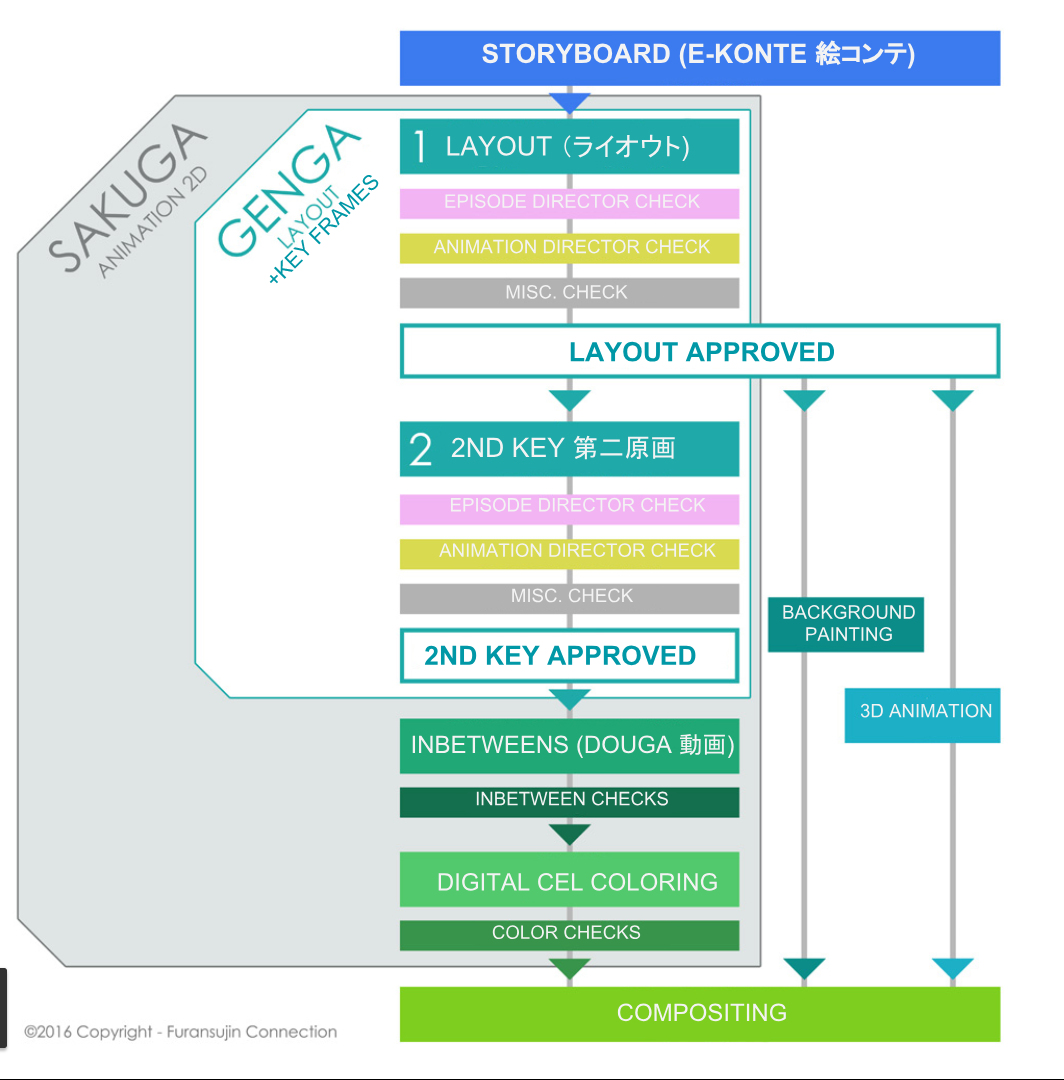
\includegraphics[width=\columnwidth]{graphics/workflow.png}
    \caption{Example of a limited animation production workflow \citep{etapes_fabrication}. The steps dealing with Sakuga (i.e., the steps following \emph{2ND KEY APPROVED} and before \emph{COMPOSITING}) are usually done using vector images.}
    \label{fig:workflow}
\end{figure}

Limited animation is an animation technique in which moving parts (or, \emph{cels}) of a drawing are reused across multiple frames. This stands in contrast to full animation, in which every frame is completely redrawn, which leads to a more fluid animation style. Hence, in order to provide a compelling experience for viewers, limited animation has to rely more on visual \emph{tricks} such as rich backgrounds (which mostly remain still within a scene and therefore can be reused).

\Cref{fig:workflow} gives an overview of the typical production process for hand-drawn limited animation. Note that since limited animation enjoys wide application in the Japanese animation industry, it contains both English and corresponding Japanese production terms. The process starts with the director creating a storyboard, which contains very rough sketches giving an overview of the animation sequence. Based on the storyboard, the key animator draws the layout (or, \emph{1st key animation}) on paper. It encompasses all keyframes in a given scene (also referred to as \emph{cut}), as well as instructions for later stages (such as camera movement). The keyframes themselves do not produce fluid animation, since they are only drawn for critical stages within an animation sequence (beginning, junctures and end). The 1st key frames already include rough sketches for the background as well as the cels. The layout is then normally checked and possibly corrected by the animation director. After the layout is approved, the rough 1st key frames are cleaned up while taking the animation director's corrections into account in order to produce 2nd key animation frames. This process can be repeated multiple times, until the animation director finally approves the keyframes.

% \begin{figure}[h]
%     \centering
%     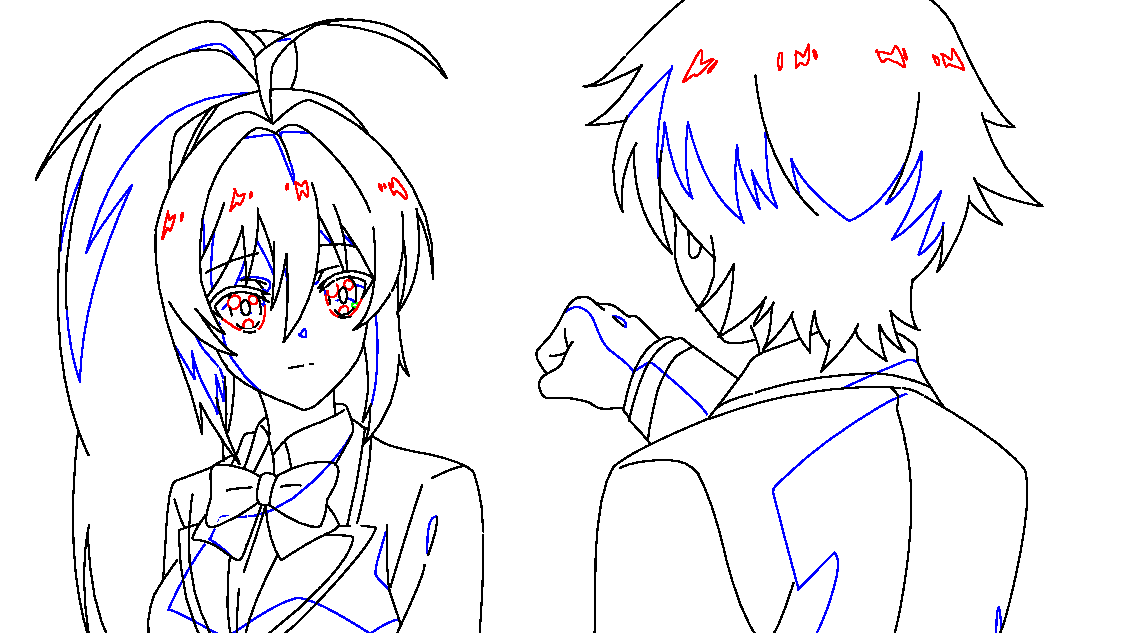
\includegraphics[width=\textwidth]{graphics/douga/39.pdf}
% %    \def\svgwidth{\columnwidth}
% %    \input{graphics/douga/49.pdf_tex}
% %    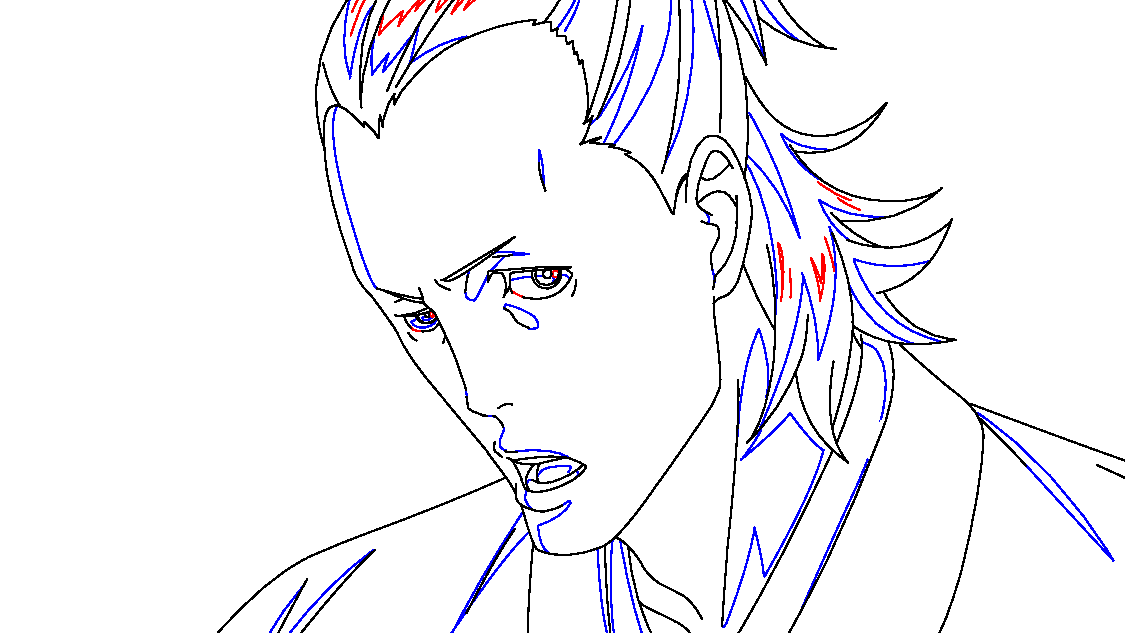
\includegraphics[]{graphics/douga/49.pdf}
% %    \includesvg[inkscapelatex=false]{graphics/douga/49.svg}
%     \caption{A clean animation keyframe in vector format. (© Tonari Animation)}
%     \label{fig:douga.example}
% \end{figure}

% \begin{figure}
%     \begin{subfigure}[b]{\textwidth}
%     \def\svgwidth{\textwidth}
%             \input{graphics/douga/48.pdf_tex}
%     \caption{Caption}
%     \end{subfigure}
%     \vfill
%     \begin{subfigure}[b]{\textwidth}
%     \def\svgwidth{\textwidth}
%             \input{graphics/douga/49.pdf_tex}
%     \caption{Caption}
%     \end{subfigure}
% \label{fig:dougaex}
% \caption{Two examples}
% \end{figure}

\begin{figure}[h!]
    \begin{subfigure}[b]{\textwidth}
    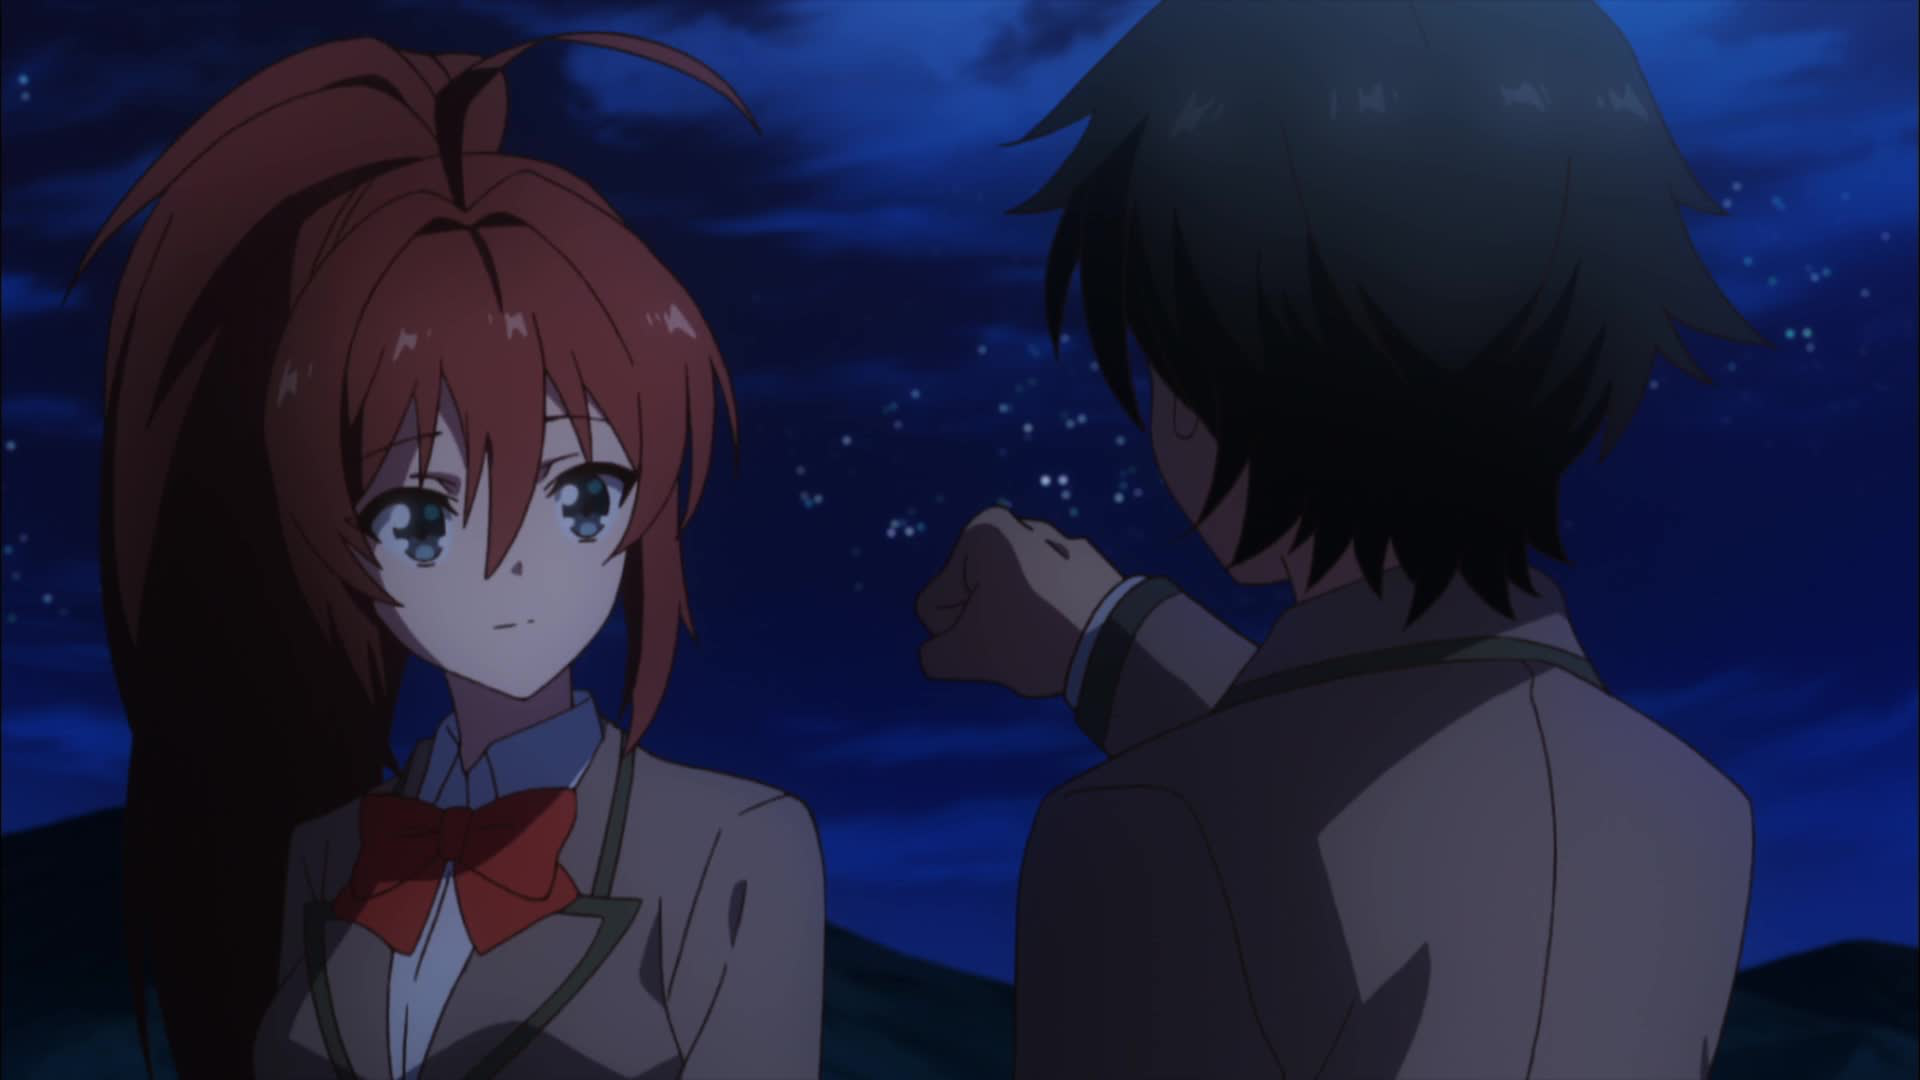
\includegraphics[width=\textwidth]{graphics/douga/39.png}
    \caption{A final composed animation frame by \citet{isekai-cheat-magician}, which is in raster format by default.}
    \label{fig:douga.example.final}
    \end{subfigure}
    \vfill
    \begin{subfigure}[b]{\textwidth}
    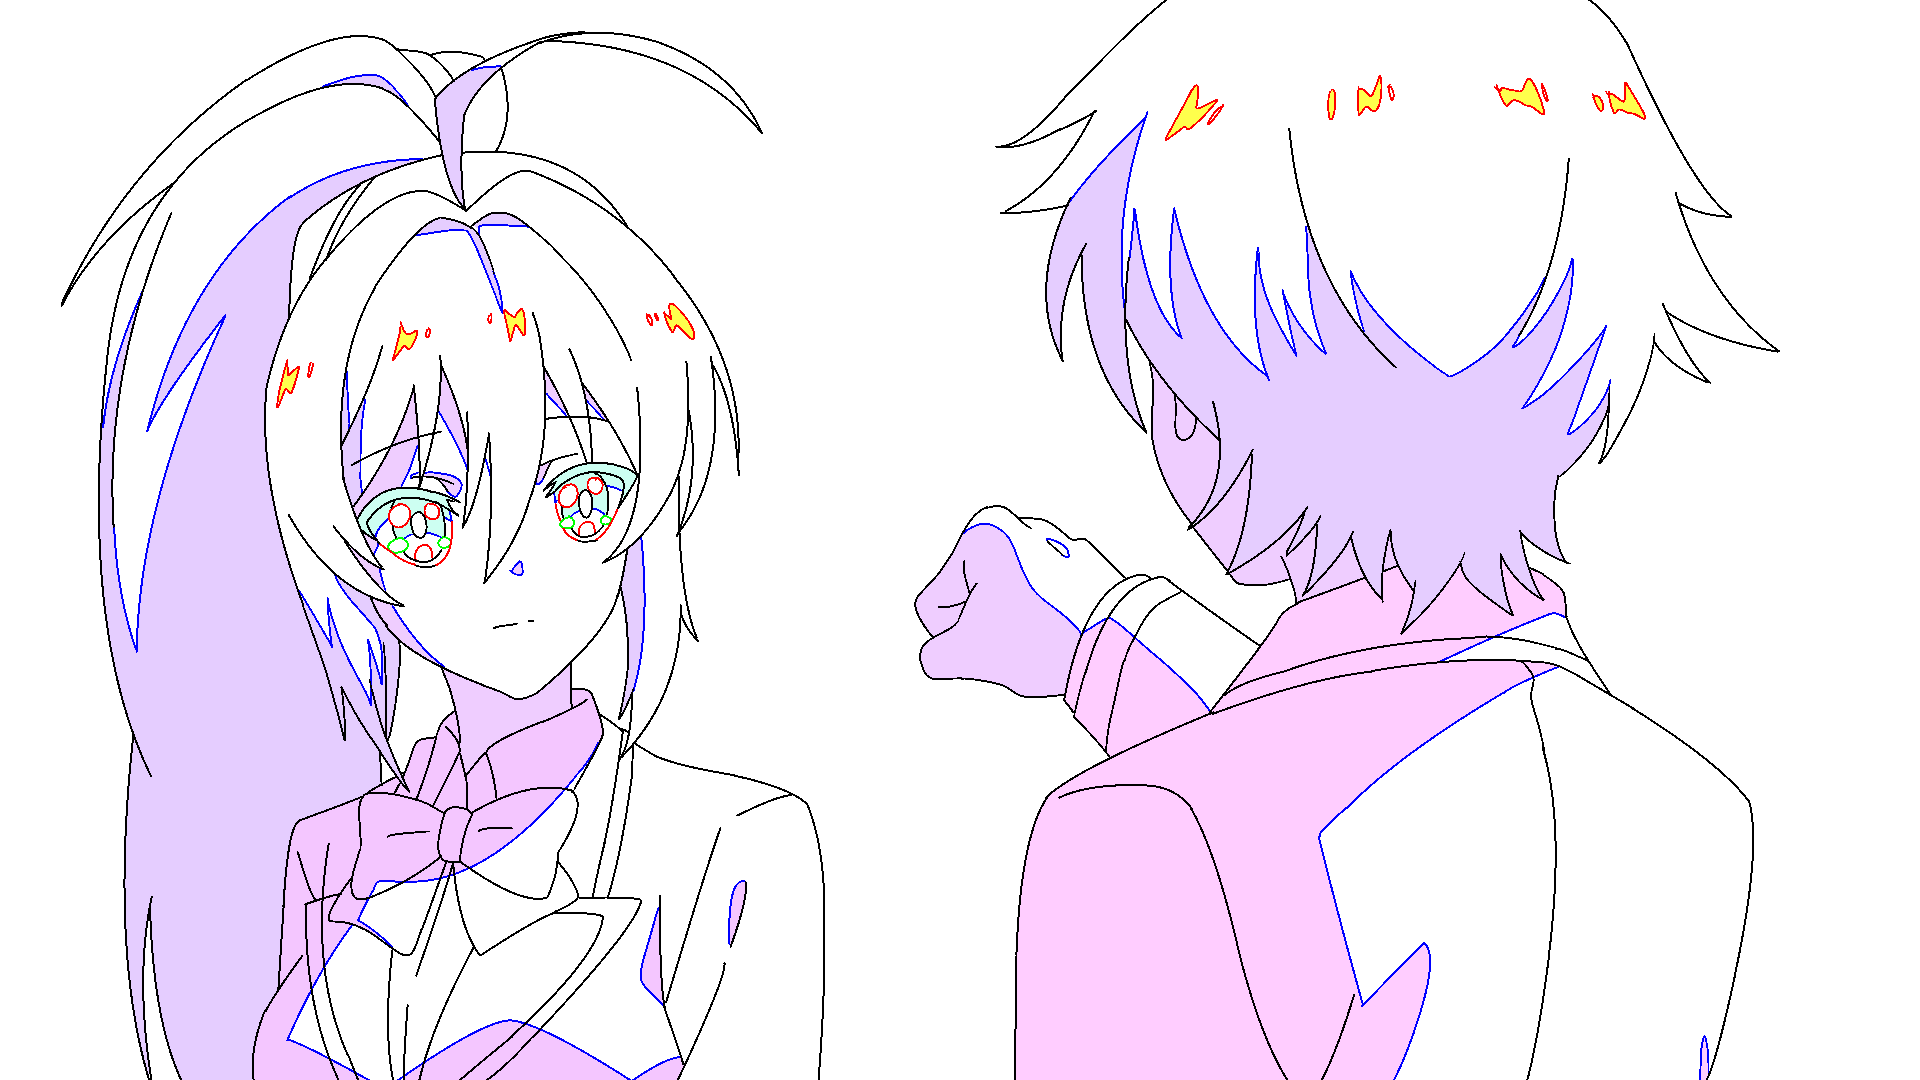
\includegraphics[width=\textwidth]{graphics/douga/836.19.png}
    \caption{The corresponding re-imagined clean animation keyframe in raster format provided by Tonari Animation.}
    \label{fig:douga.example.clean}
    \end{subfigure}
\caption{An example of a clean animation keyframe and the corresponding final animation frame.}
\label{fig:douga.example}
\end{figure}


Afterwards, the approved keyframes are retraced and digitized as vector images. These clean final frames are not full drawings, but include the outlines of each object in a scene, decorative lines, as well as lines indicating shadows, lighting and color regions. It can be interpreted as a semantic description of the essential parts (mostly cels) of the final frame. An example can be seen in \Cref{fig:douga.example.clean}. 

The keyframes are retraced as vector images since this format makes it easy to apply succeeding steps in the workflow. Vector images can be easily and accurately edited by simply altering primitives. Furthermore, images are often worked on at different scales, where the resolution-independent nature of vector images is beneficial. This is especially important when working on tiny details of the image.

\begin{figure}[h]
    \begin{subfigure}[b]{0.3\textwidth}
    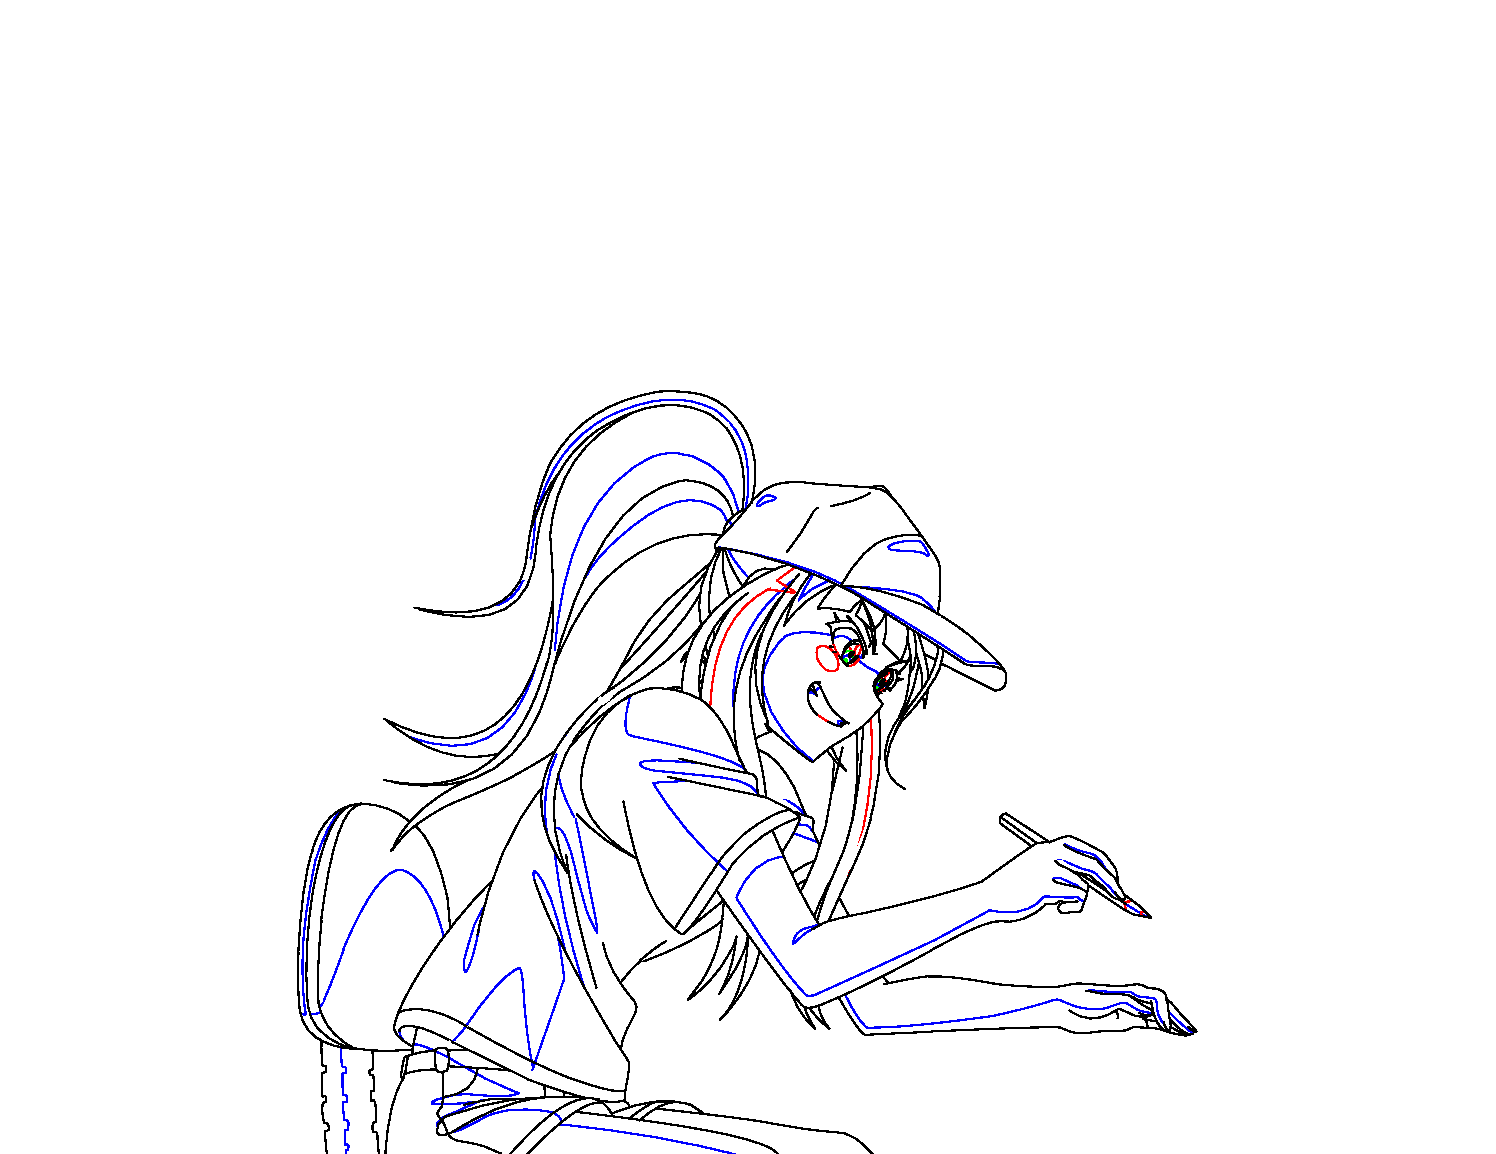
\includegraphics[width=\textwidth]{graphics/douga/007AD_DOU_26.pdf}
    \end{subfigure}
    \begin{subfigure}[b]{0.3\textwidth}
    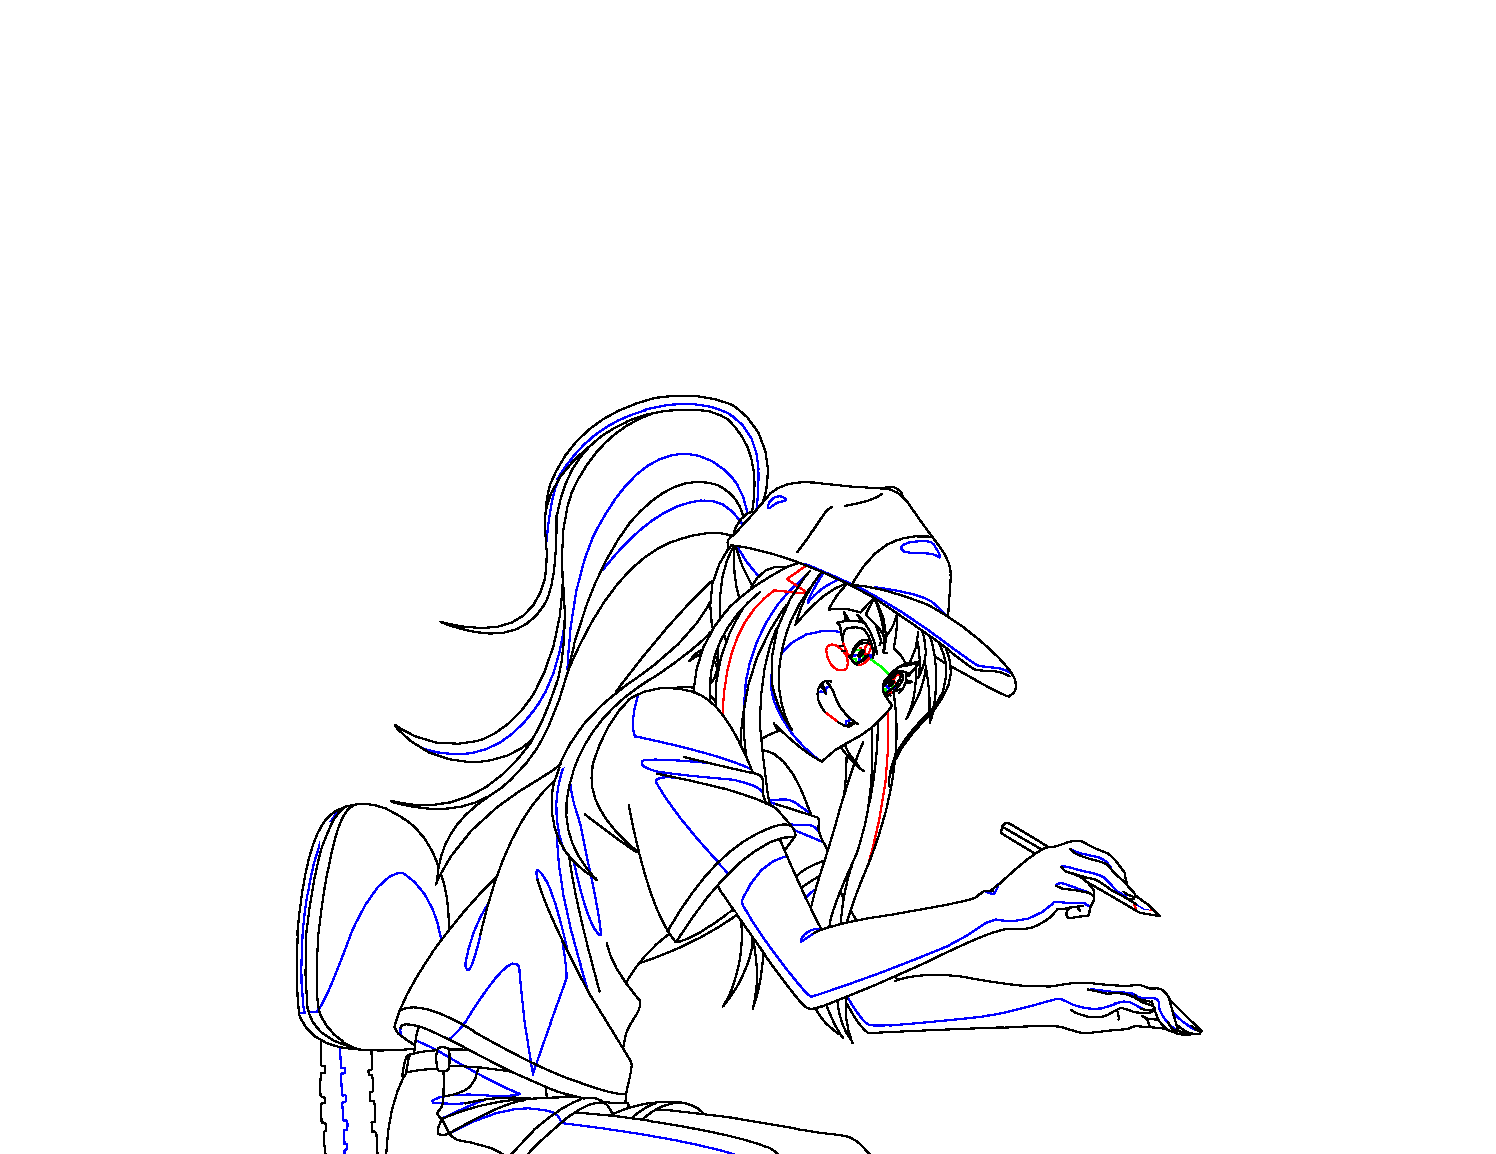
\includegraphics[width=\textwidth]{graphics/douga/007AD_DOU_27.pdf}
    \end{subfigure}
    \begin{subfigure}[b]{0.3\textwidth}
    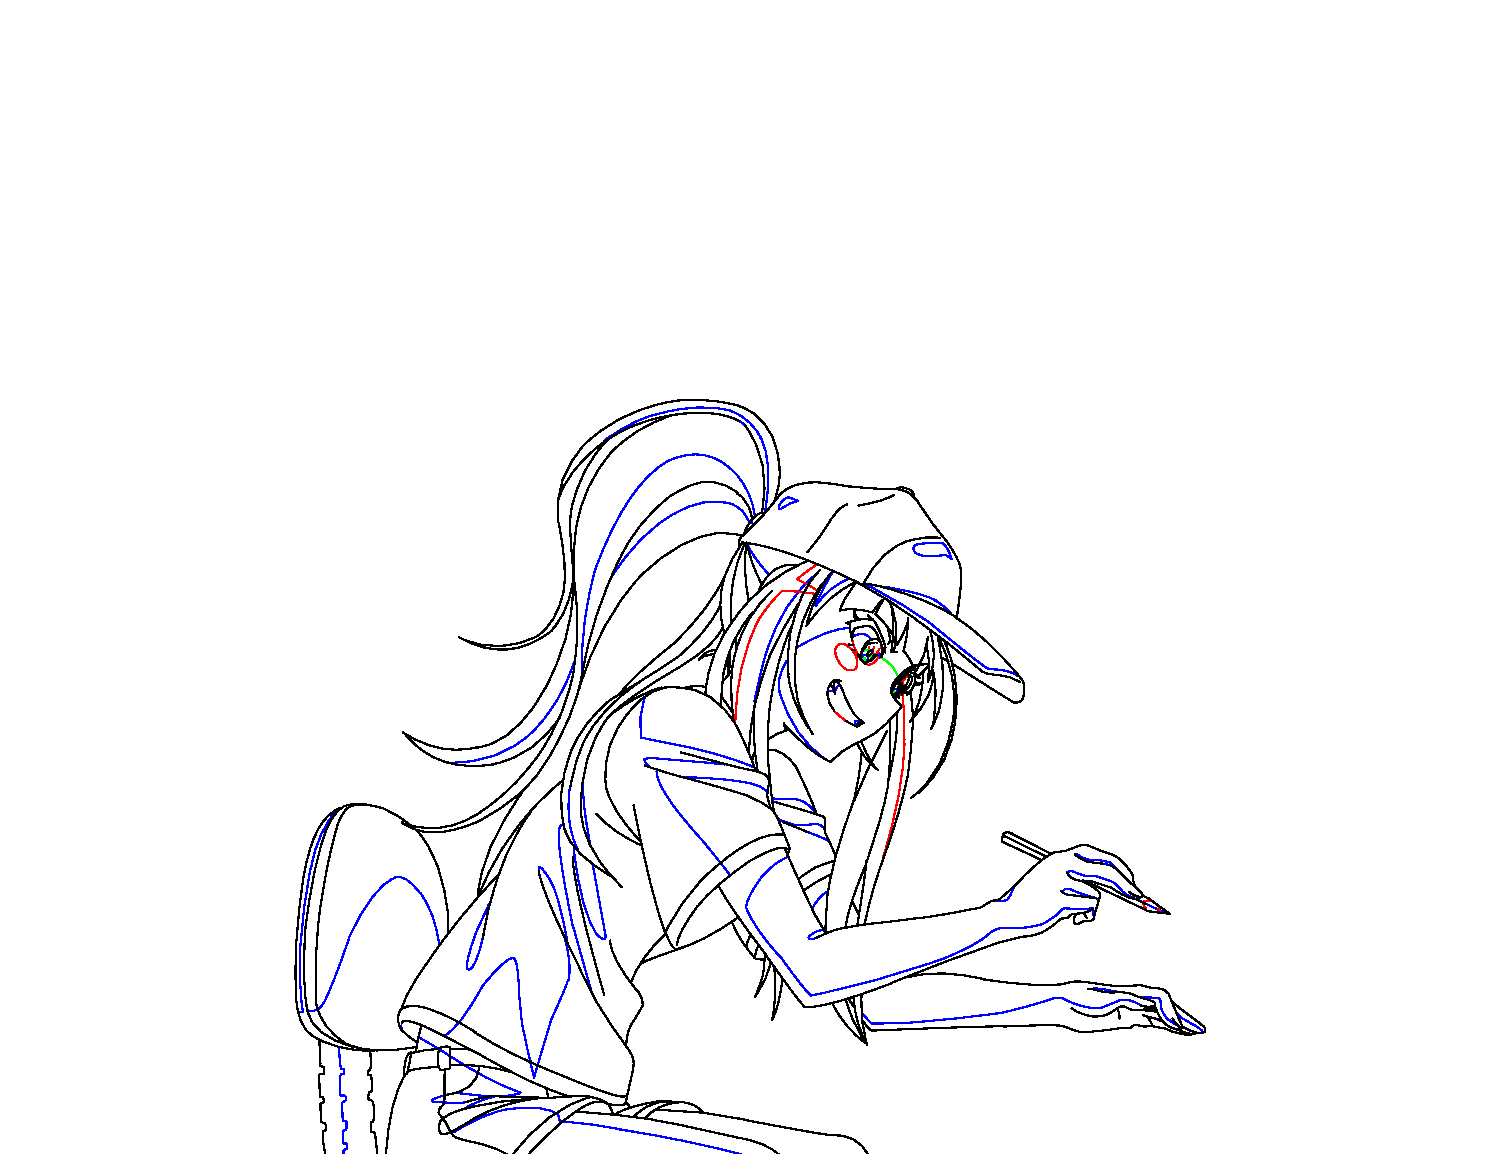
\includegraphics[width=\textwidth]{graphics/douga/007AD_DOU_28.pdf}
    \end{subfigure}
\caption{Three successive clean frames of an animation scene in vector format provided by Tonari Animation. If rapidly shown in succession, the person appears to be moving. Notice minor differences among them, such as the angle of the pencil or the location of strains of hair.}
\label{fig:multiple-douga}
\end{figure}

While up to now only keyframes were drawn, in order to produce fluid movement between them, \emph{inbetweens} are created using the clean keyframes as reference. This is done at such a late stage in order to speed up the process (since only keyframes need to be revised and refined in the initial steps as opposed to all frames). Inbetweens need to be drawn exactly like the keyframe, while having small deviations for moving parts. For the workflow succeeding this step, there is no distinction between keyframes and inbetweens anymore. The resulting images are referred to by various terms interchangeably; most consistently used is the term \emph{douga} (\begin{CJK}{UTF8}{min}動画\end{CJK}, lit. \emph{moving image}) in Japanese limited animation production. \Cref{fig:multiple-douga} depicts three examples of \emph{douga}.

After the clean frames are drawn and approved, they are colored according to their color indications. The color indications in the key animations serve to retain temporal consistency for the coloring. Nowadays, this is done digitally using bucket filling, i.e., changing the color within a closed area in the image. The precise nature of the vector image makes this process easier, since there is no ambiguity where exactly color areas are located. Since the resulting animation video will be displayed on raster displays at a fixed resolution, for succeeding steps it is not necessary for the frames to be in vector format anymore. Hence, they are rasterized and composited with the background, which was drawn in parallel in raster format. While in theory, clean frames could be rasterized at any arbitrary size, usually, they are rasterized with a width of 720 pixels. Finally, camera movement, special effects, 3-D animation and small fixes are added. An example of such a final frame is depicted in \Cref{fig:douga.example.final}. 


\subsection{Clean Frames}
\label{subsec:cleanframes}

\begin{figure}
        \begin{subfigure}[b]{0.4\textwidth}
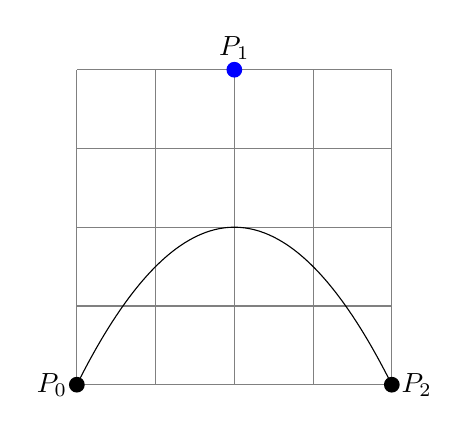
\begin{tikzpicture}
    \draw[color=gray] (0,0) grid (4,4);
    \coordinate (A) at (0,0);
    \coordinate (B) at (1.333,2.667);
    \coordinate (C) at (2.667,2.667);
    \coordinate (D) at (4,0);
    \coordinate (E) at (2,4);
    \fill (A) circle (0.1) node[left]{$P_0$};
    \fill[blue] (E) circle (0.1) node[above, color=black]{$P_1$};
    \fill (D) circle (0.1) node[right]{$P_2$};
    \draw[black] (A)..controls (B) and (C) .. (D);
\end{tikzpicture}
    \caption{A quadratic bezier curve, defined by a start point $P_0$, an end point $P_2$ and one control point $P_1$.}
    \end{subfigure}
    \hfill
    \begin{subfigure}[b]{0.4\textwidth}
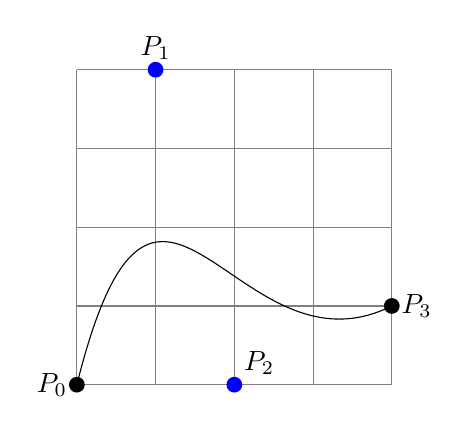
\begin{tikzpicture}
    \draw[color=gray] (0,0) grid (4,4);
    \coordinate (A) at (0,0);
    \coordinate (B) at (1,4);
    \coordinate (C) at (2,0);
    \coordinate (D) at (4,1);
    \fill (A) circle (0.1) node[left]{$P_0$};
    \fill[blue] (B) circle (0.1) node[above, color=black]{$P_1$};
    \fill[blue] (C) circle (0.1) node[above right, color=black]{$P_2$};
    \fill (D) circle (0.1) node[right]{$P_3$};
    \draw[black] (A)..controls (B) and (C) .. (D);
\end{tikzpicture}
    \caption{A cubic bezier curve, defined by a start point $P_0$, an end point $P_3$ and two control points $P_1$ and $P_2$.}
    \end{subfigure}
    \caption{Examples of bezier curves.}
    \label{fig:bezier-example}
\end{figure}

The focus of this work are the clean frames as used in the production workflow after the 2nd key animation and prior to the coloring, as shown in \Cref{fig:douga.example.clean}. Digital clean frames are primarily drawn using \emph{bezier curves} \citep{de1986formes} as graphical primitive. Bezier curves are smooth parametric functions that approximate real-world strokes. \Cref{fig:bezier-example} gives two examples of bezier curves. They are parameterized by a start and an end point, as well as a variable number of control points. The curve is then constructed using a combination of linear interpolations between the points. The number of control points indicates the degree of the curve; most commonly used are \emph{quadratic} and \emph{cubic} bezier curves, as nearly all relevant shapes can be represented using them. Note, that a bezier curve of degree $n$ can also be represented by a bezier curve of degree $m>n$. Furthermore, every bezier curve can be split at any point into two bezier curves of the same degree.

\begin{figure}[!h]
    \centering
    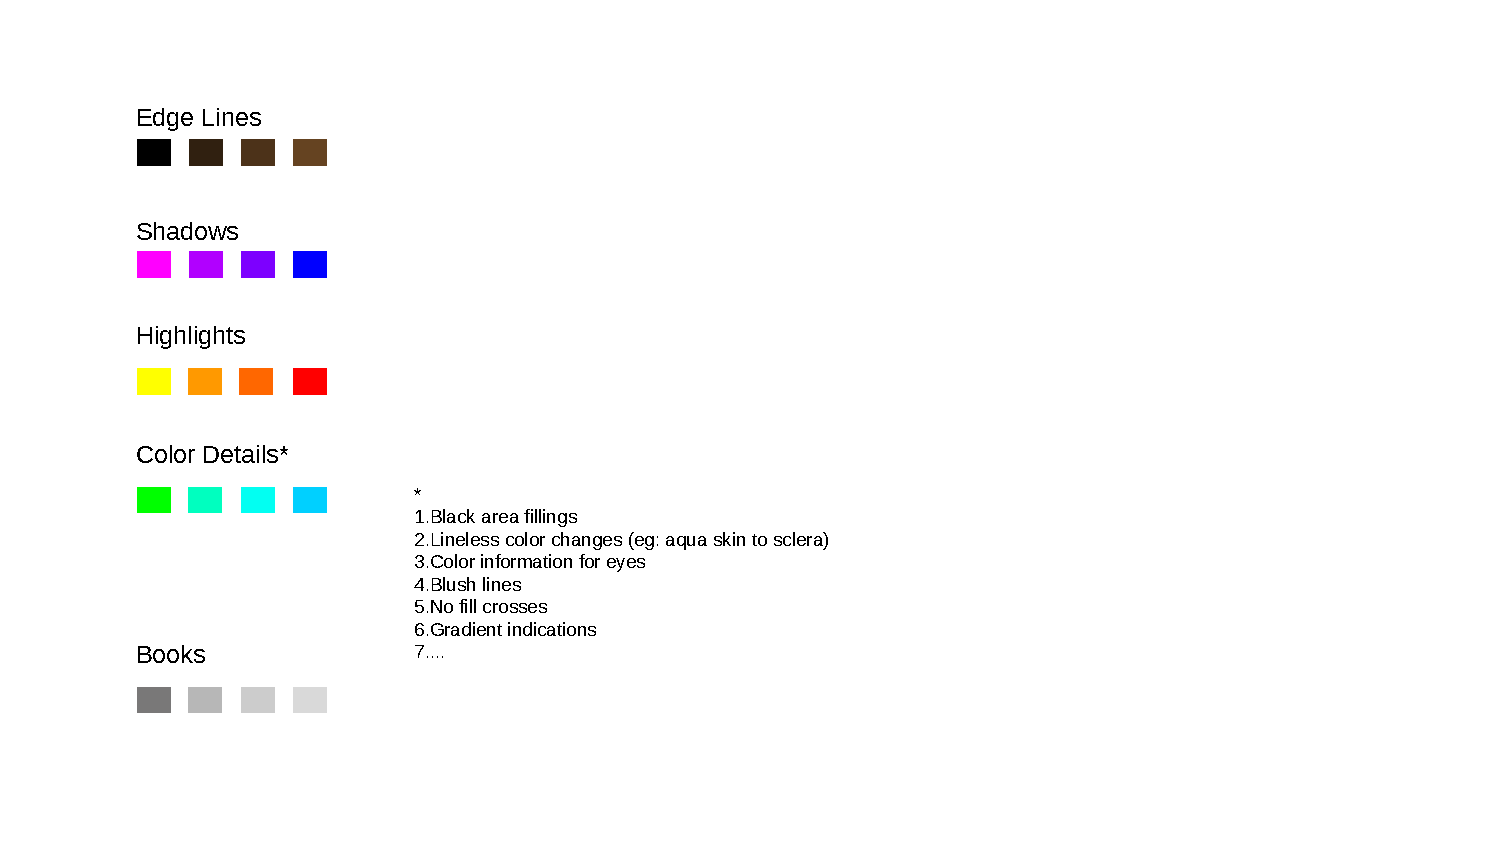
\includegraphics{graphics/Douga-Color-Schema.pdf}
    \caption{Our proposed standardized keyframe color schema, which is used in the dataset \citep{Kugler-2021}.}
    \label{fig:bg.color-schema}
\end{figure}

Clean frames can be considered a type of line art, specifically defined by the following features.

\begin{itemize}
    \item Constant stroke width: Clean frames are drawn using mostly quadratic and cubic bezier curves with a constant stroke width. While line art usually uses variable stroke widths, this is not a common style for limited animation, specifically in Japanese productions. 
    \item High number of curves:  On average, the amount of curves per image over 1000 (see \Cref{subsec:dataset.stats}), which is significantly more than the amount of curves used for simple line art that is often the target for automatic vectorization (such as doodles, fonts or cartoons).
    \item Semantically meaningful colors: The color of each curve carries semantic meaning, namely as indication for succeeding steps in the animation pipeline. There is no industry-standard for the color scheme, with studios mostly opting to use their proprietary schemes. The scheme used by example images in this work (all provided by Tonari Animation) is defined in \Cref{fig:bg.color-schema}. It can be observed in \Cref{fig:douga.example}. For example, note how the regions enclosed by blue lines are colored darker than the ones enclosed by red lines.
    \item Exact boundaries: In order to speed up the colorization step of the production workflow, it is necessary to ensure that all color regions are sufficiently enclosed by curves. This way, coloring can be trivially accomplished using bucket filling.
\end{itemize}

Even if clean frames are drawn as vector images, they might sometimes only be available in raster format. This could be the case of older clean frames, different studios working on different stages of the workflow or if it is necessary to export the image from the drawing program to another program. In this case, they need to be manually retraced before inbetweens are created, which can take around an hour. Hence, there is a need to have an automatic way of vectorizing them.

\begin{figure}[h]
    \centering
    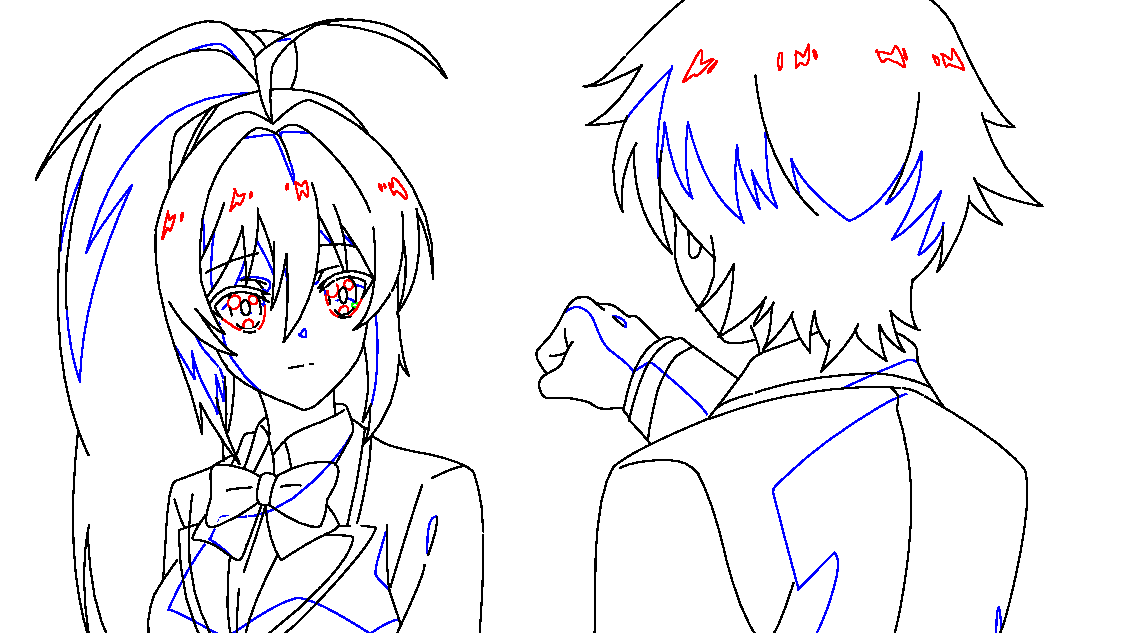
\includegraphics[width=\textwidth]{graphics/douga/39.pdf}
    \caption{The essential information of a clean animation keyframe. In essence, \Cref{fig:douga.example.clean} with all filled color regions removed.}
    \label{fig:clean-frame-vec}
\end{figure}

The objective of this work is to create an automatic way of vectorizing clean frames. For the vectorization, it is not necessary to handle the filled color regions, since those can be easily restored using pre- or post-processing and, failing that, can be trivially added manually. The essential part are the lines and curves themselves, as shown in \Cref{fig:clean-frame-vec}. %Furthermore, it is not necessary for the algorithm itself to restore curves in their correct color, since the image can easily be split automatically according to the color. Then, the vectorization algorithm can be applied on each of the resulting partial images. Afterwards, the partial results can be trivially colored and merged.

Finally, in order for the vectorization method to be practically suitable, it is important that the result minimizes the amount of manual fixing required. Hence, it is more important that the restored lines are correct, even at the expense of not all lines in the input image being covered.
